
%(BEGIN_QUESTION)
% Copyright 2011, Tony R. Kuphaldt, released under the Creative Commons Attribution License (v 1.0)
% This means you may do almost anything with this work of mine, so long as you give me proper credit

Pressure transmitter PT-89 on this natural gas separator vessel presently has a calibrated range of 0 to 400 PSIG.  Operations personnel would like you to re-range this transmitter for 300 to 375 PSIG instead:

$$\includegraphics[width=15.5cm]{i0003rx01.eps}$$

Answer the following questions about the task of re-ranging, explaining each of your answers:

\begin{itemize}
\item{} Does the new, requested range constitute a {\it zero} shift, a {\it span} shift, or both?
\vskip 10pt
\item{} If this is a ``smart'' (digital) transmitter, does it need to be {\it re-trimmed} as well as {\it re-ranged}?
\vskip 10pt
\item{} Will the control room indicator PIR-89 need to be {\it re-calibrated}, {\it re-ranged}, or both?
\vskip 10pt
\item{} Will the local pressure gauge PG-131 need to be {\it re-calibrated} as well?
\vskip 10pt
\item{} Will the pressure safety valves PSV-11, PSV-12, and/or PSV-13 need to be set for lower ``lift'' pressures?
\vskip 10pt
\item{} If the maximum (factory) range of this pressure transmitter is 0 to 750 PSI and the maximum turndown ratio for the required accuracy is 20:1, will it be able to meet the new range?  If not, what might you have to do in order to fulfill operations' request?
\vskip 10pt
\item{} Why do you suppose operations would like you to re-range this transmitter?  In other words, what operational advantage(s) might be gained from doing so?  Are there any potential disadvantages of having the new range versus the old?
\end{itemize}

\underbar{file i03524}
%(END_QUESTION)





%(BEGIN_ANSWER)


%(END_ANSWER)





%(BEGIN_NOTES)

\begin{itemize}
\item{} Does the new, requested range constitute a {\it zero} shift, a {\it span} shift, or both?  {\bf This is both a zero shift (LRV from 0 to 300) and a span shift (span from 400 to 75).}
\vskip 10pt
\item{} If this is a ``smart'' (digital) transmitter, does it need to be {\it re-trimmed} as well as {\it re-ranged}?  {\bf No.}
\vskip 10pt
\item{} Will the control room indicator PIR-89 need to be {\it re-calibrated}, {\it re-ranged}, or both? {\bf PIR-89 will need to be re-ranged as well, but not (necessarily) re-calibrated.  PIR-89 needs to display different pressure values for its 4-20 mA input, but presumably it is still capable of accurately interpreting 4 mA and 20 mA so no re-calibration is necessary.}
\vskip 10pt
\item{} Will the local pressure gauge PG-131 need to be {\it re-calibrated} as well?  {\bf No, because its operation is completely independent of PT-89 and PIR-89.}
\vskip 10pt
\item{} Will the pressure safety valves PSV-11, PSV-12, and/or PSV-13 need to be set for lower ``lift'' pressures? {\bf Again, no, because these valves' operation are independent of the pressure transmitter loop.  Safety valves are always rated by the pressure limits of the vessel(s), just as electrical fuses are rated by the current the wires can handle.}
\vskip 10pt
\item{} If the maximum (factory) range of this pressure transmitter is 0 to 750 PSI and the maximum turndown ratio for the required accuracy is 20:1, will it be able to meet the new range?  If not, what might you have to do in order to fulfill operations' request? {\bf The turndown ratio of 20:1 means the minimum span can be set all the way down to 37.5 PSI.  Since operations is requesting a 75 PSI span, you should be alright.}
\vskip 10pt
\item{} Why do you suppose operations would like you to re-range this transmitter?  In other words, what operational advantage(s) might be gained from doing so?  Are there any potential disadvantages of having the new range versus the old? {\bf Reducing the pressure measurement range results in the recorder's graphical display showing more detail (resolution) within the range of 300 to 375 PSI.  Pressure changes which would have formerly shown up as tiny wiggles in the trend may now be seen in far greater detail because the vertical axis of the trend has been essentially magnified by the span change.}
\end{itemize}






\vskip 20pt \vbox{\hrule \hbox{\strut \vrule{} {\bf Virtual Troubleshooting} \vrule} \hrule}

This question is a good candidate for a ``Virtual Troubleshooting'' exercise.  Presenting the diagram to students, you first imagine in your own mind a particular fault in the system.  Then, you present one or more symptoms of that fault (something noticeable by an operator or other user of the system).  Students then propose various diagnostic tests to perform on this system to identify the nature and location of the fault, as though they were technicians trying to troubleshoot the problem.  Your job is to tell them what the result(s) would be for each of the proposed diagnostic tests, documenting those results where all the students can see.

During and after the exercise, it is good to ask students follow-up questions such as:

\begin{itemize}
\item{} What does the result of the last diagnostic test tell you about the fault?
\item{} Suppose the results of the last diagnostic test were different.  What then would that result tell you about the fault?
\item{} Is the last diagnostic test the best one we could do?
\item{} What would be the ideal order of tests, to diagnose the problem in as few steps as possible?
\end{itemize}

%INDEX% Calibration, electronic pressure transmitter: zero and span adjustments
%INDEX% Calibration, smart transmitter: digital trim
%INDEX% Calibration, turndown: applied to pressure transmitter application
%INDEX% Process: gas compressor inlet separator (realistic P&ID shown)

%(END_NOTES)

